% Options for packages loaded elsewhere
\PassOptionsToPackage{unicode}{hyperref}
\PassOptionsToPackage{hyphens}{url}
%
\documentclass[
]{article}
\usepackage{lmodern}
\usepackage{amssymb,amsmath}
\usepackage{ifxetex,ifluatex}
\ifnum 0\ifxetex 1\fi\ifluatex 1\fi=0 % if pdftex
  \usepackage[T1]{fontenc}
  \usepackage[utf8]{inputenc}
  \usepackage{textcomp} % provide euro and other symbols
\else % if luatex or xetex
  \usepackage{unicode-math}
  \defaultfontfeatures{Scale=MatchLowercase}
  \defaultfontfeatures[\rmfamily]{Ligatures=TeX,Scale=1}
\fi
% Use upquote if available, for straight quotes in verbatim environments
\IfFileExists{upquote.sty}{\usepackage{upquote}}{}
\IfFileExists{microtype.sty}{% use microtype if available
  \usepackage[]{microtype}
  \UseMicrotypeSet[protrusion]{basicmath} % disable protrusion for tt fonts
}{}
\makeatletter
\@ifundefined{KOMAClassName}{% if non-KOMA class
  \IfFileExists{parskip.sty}{%
    \usepackage{parskip}
  }{% else
    \setlength{\parindent}{0pt}
    \setlength{\parskip}{6pt plus 2pt minus 1pt}}
}{% if KOMA class
  \KOMAoptions{parskip=half}}
\makeatother
\usepackage{xcolor}
\IfFileExists{xurl.sty}{\usepackage{xurl}}{} % add URL line breaks if available
\IfFileExists{bookmark.sty}{\usepackage{bookmark}}{\usepackage{hyperref}}
\hypersetup{
  pdftitle={Final Report},
  pdfauthor={Brandyn Ruiz},
  hidelinks,
  pdfcreator={LaTeX via pandoc}}
\urlstyle{same} % disable monospaced font for URLs
\usepackage[margin=1in]{geometry}
\usepackage{longtable,booktabs}
% Correct order of tables after \paragraph or \subparagraph
\usepackage{etoolbox}
\makeatletter
\patchcmd\longtable{\par}{\if@noskipsec\mbox{}\fi\par}{}{}
\makeatother
% Allow footnotes in longtable head/foot
\IfFileExists{footnotehyper.sty}{\usepackage{footnotehyper}}{\usepackage{footnote}}
\makesavenoteenv{longtable}
\usepackage{graphicx,grffile}
\makeatletter
\def\maxwidth{\ifdim\Gin@nat@width>\linewidth\linewidth\else\Gin@nat@width\fi}
\def\maxheight{\ifdim\Gin@nat@height>\textheight\textheight\else\Gin@nat@height\fi}
\makeatother
% Scale images if necessary, so that they will not overflow the page
% margins by default, and it is still possible to overwrite the defaults
% using explicit options in \includegraphics[width, height, ...]{}
\setkeys{Gin}{width=\maxwidth,height=\maxheight,keepaspectratio}
% Set default figure placement to htbp
\makeatletter
\def\fps@figure{htbp}
\makeatother
\setlength{\emergencystretch}{3em} % prevent overfull lines
\providecommand{\tightlist}{%
  \setlength{\itemsep}{0pt}\setlength{\parskip}{0pt}}
\setcounter{secnumdepth}{-\maxdimen} % remove section numbering

\title{Final Report}
\author{Brandyn Ruiz}
\date{}

\begin{document}
\maketitle

\hypertarget{introduction}{%
\section{Introduction}\label{introduction}}

With the recent events of covid cases on the rise and steadly holding
just barely and with the rise of fires all over California with the sky
being orange miles away from the fire for days, this year has definitely
been so unusual and unprecedented times. The Corona virus has been found
to inhibit respiratory functions of the host and with the recent fires
the air quality within many cities of the 58 counties has sky rocketed
to concerning levels. Depending on someone's geographical location and
which county they live in, their health could already be at risk due to
the air quality alone. Would this make a subject more vulnerable to
contracting covid if their respiratory function was already inhibited?
My hypothesis that I want to further explore is whether there is an
association between air quality and confirmed cases of covid amongst
people within the counties of California.

\hypertarget{methods}{%
\section{Methods}\label{methods}}

The data sets that I have used in my analysis were from three different
extrenal sources consisting of John Hopkins University's github
repository of
\href{\%22https://raw.githubusercontent.com/CSSEGISandData/COVID-19/master/csse_covid_19_data/csse_covid_19_time_series/time_series_covid19_confirmed_US.csv\%22}{daily
covid cases} by geolocation. The github repository has different
datasets of deaths and confirmed cases within the United States from the
corona virus and is a compilation from news article sources such as New
York Times and Los Angeles Times, as well as Public Health departments
of the different counties. Daily Air Quality Index and PM 2.5
concentrations were from the
\href{https://www.epa.gov/outdoor-air-quality-data/download-daily-data}{Enviornmental
Protection Agency (EPA)}. Air Quality Index is measured on a scale from
0 to 500, where it measures the change of pollution in the air, see the
figure below to reference the different cutoffs and categories we
usually see on our weather and map applications on our phones. PM 2.5
pollutants are small microscopic particles within the air such as dust,
spores, pollen, and ash which measure about 2.5 \(\mu\)m (micrometers)
in diameter. Within the EPA's website I queried for my own results for
all recording sites within the state of interest being California as PM
2.5 being the pollutant. I have found that the query directly from the
EPA's website was much more accurate and updated more frequently than
downloading their daily datasets through their API. I have also gathered
\href{https://www.census.gov/data/tables/time-series/demo/popest/2010s-counties-detail.html}{US
Census data} of predicted 2019 estimates of populations, gender, and
race within every county in California.

\begin{figure}
\centering
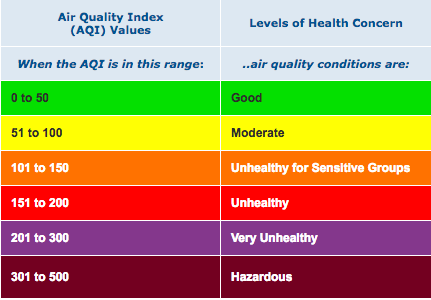
\includegraphics{data/air-quality-alerts.png}
\caption{Air Quality Figure}
\end{figure}

\hypertarget{daily-covid-cases}{%
\subsection{Daily Covid Cases}\label{daily-covid-cases}}

In data wrangling and cleaning the daily covid data we were originally
provided 60 observations 1 observation for each county. However, there
are only 58 total counties within California, looking more into this the
covid dataset has included people who were from `unassigned' counties
and `Out of CA', which could represent NA or an omitted response from
the person who contracted the virus as well as people who tested
positive within California, but are not a resident of California. I have
exluded these observations to be exlusive corona virus cases within
California for easier match of datasets between counties. We also
observe from the raw csv file is that the data is recorded for each day
across every county and each new day is a column, with a total of 319
columns as of 11/25 which is reporting data from the previous day. To
match a very wide dataset to others such as the AQI from the EPA's
website it needs to be transformed into a longitidinal dataset with
dates as columns and the value of covid cases falling into that day as
its own value column which is labeled as \texttt{Confirmed} for total
confirmed cases. This was eaily done by using the \texttt{melt()}
function which we kept our other variables as our ID factors with
\texttt{Date} being transformed into the new column and chronologically
ordered by each county. Our raw dataset is the grand total of cases
since the beginning of the pandemic, a grand total accumulation of cases
up until that particular date. This particular variable of
\texttt{Confirmed} cases would cause overinflation and I have made a for
loop to iterate for each date for every county, taking the subtraction
of current covid cases from the previous day to get the incidence or
\texttt{new\_cases} for that day. As we see in \emph{Figure 1} the green
line represents Los Angeles county and has the largest spike and
cyclical trends compared to the other counties. Population of Los
Angeles county could be a huge factor in why such a huge difference in
cases. A better reference is on my website homepage with interactive
text of county and incidence cases. What sticks out the most is the blue
line going past the 0 y-axis, which indicates that San Bernadino county
had the largest difference from the previous day where there was fewer
reported cases. This trend is what we hope to see in the nearby future.

\textbf{Figure 1: Incidence Cases Across the Pandemic}
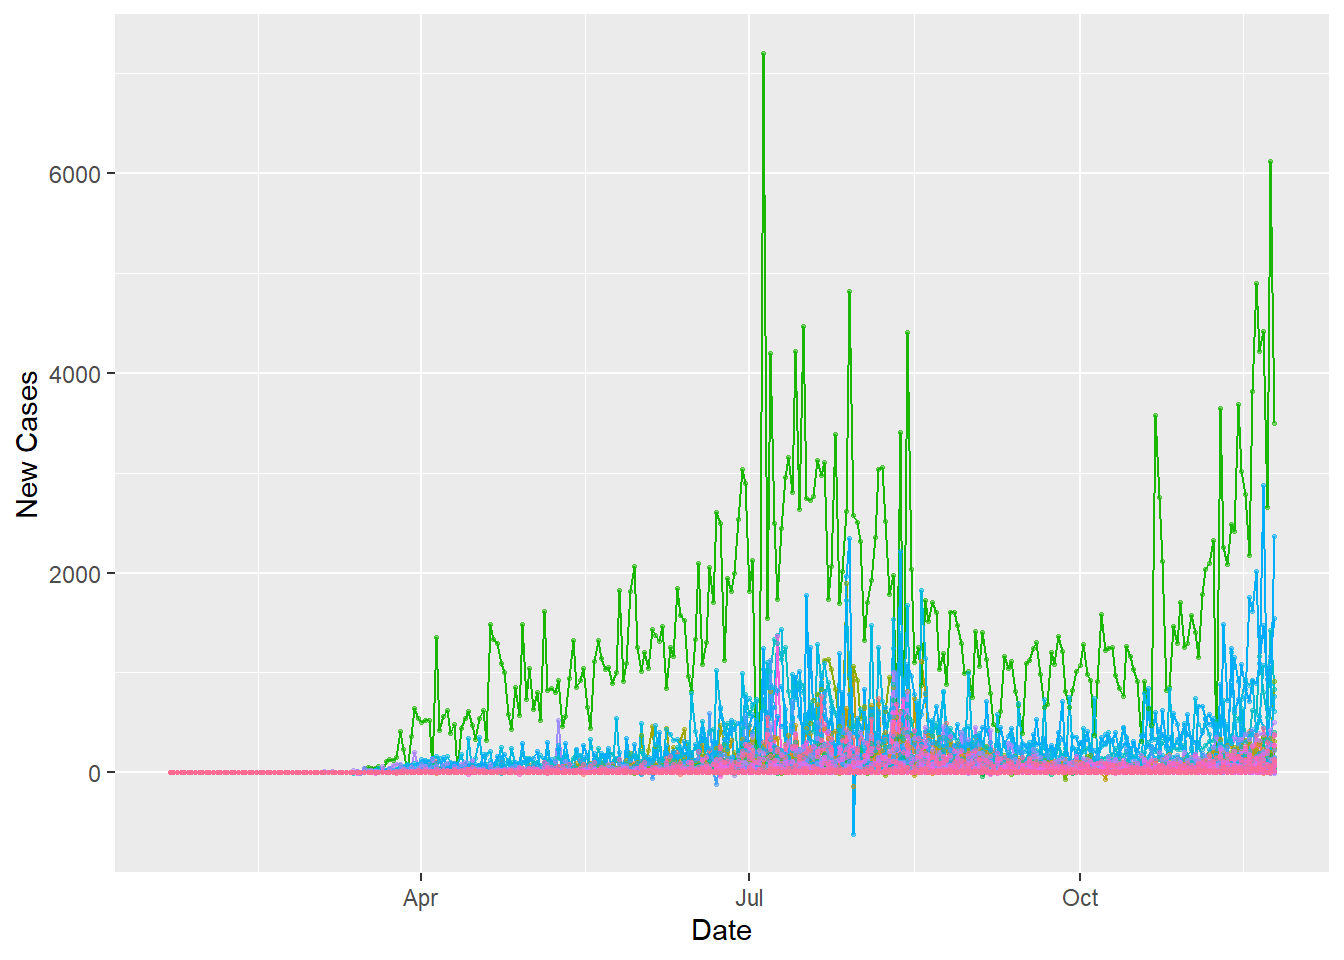
\includegraphics{FinalReport_files/figure-latex/COVID Visual by County-1.pdf}

\textbf{Figure 2: Incidence Cases}
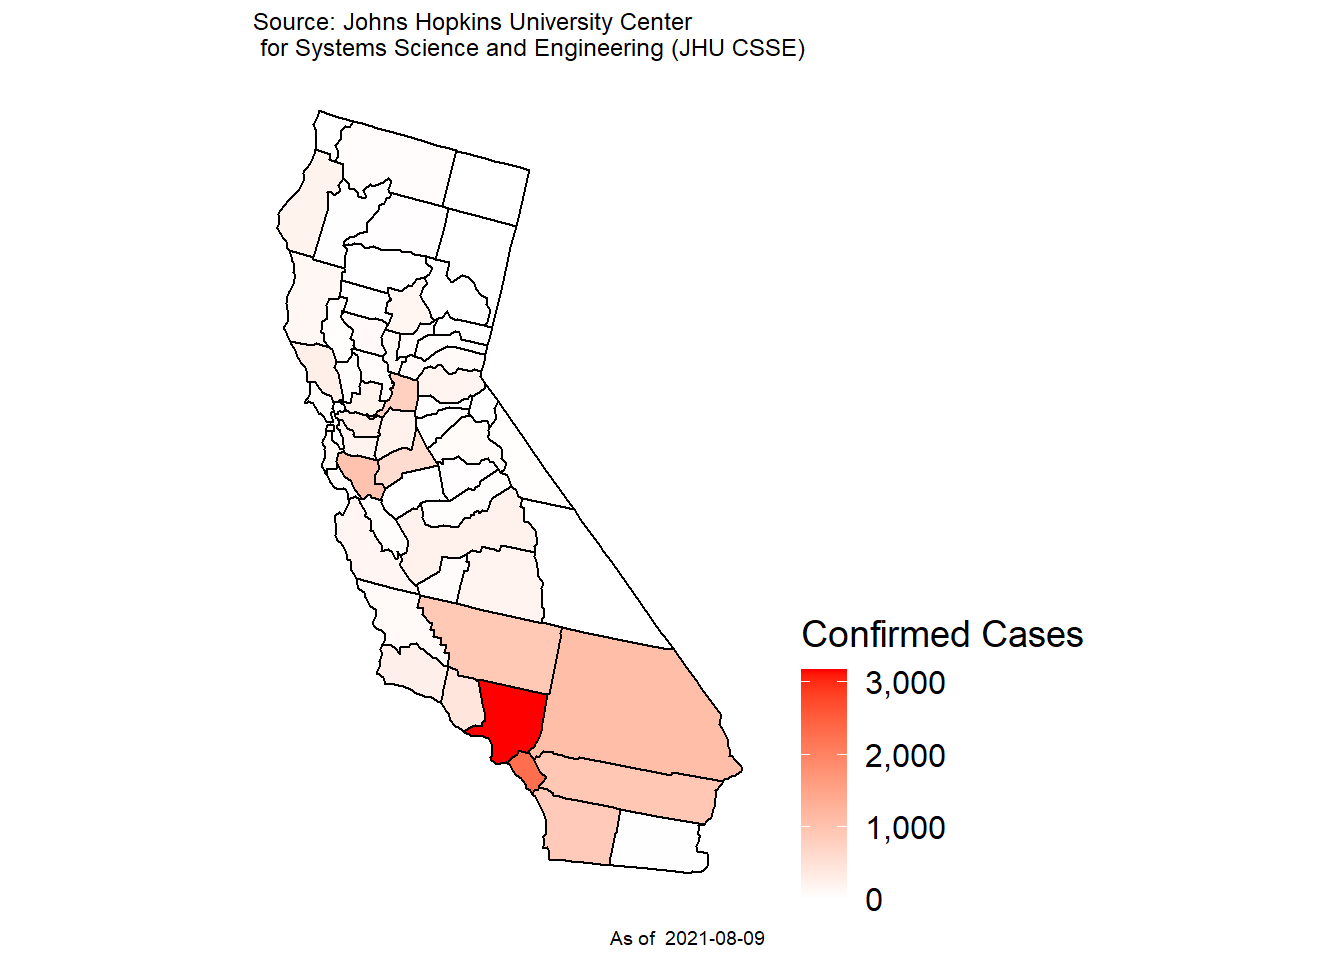
\includegraphics{FinalReport_files/figure-latex/Spatial Visualization of COVID by County-1.pdf}

\textbf{Figure 3: Prevalence of Confirmed Cases}
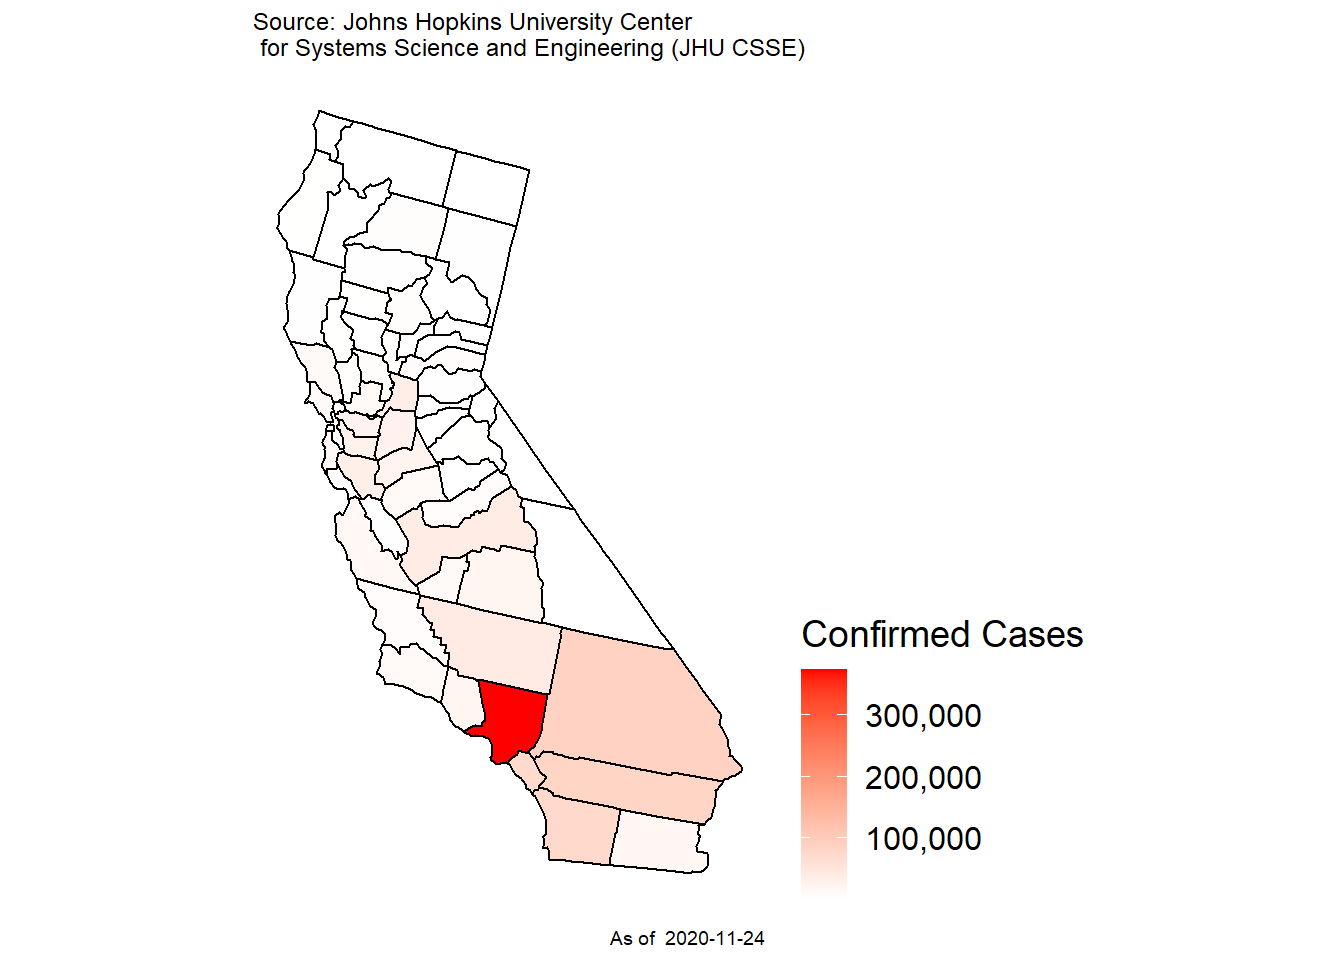
\includegraphics{FinalReport_files/figure-latex/Grand Total Confirmed Cases-1.pdf}

Our daily cases dataset also provides the \texttt{FIPS} or Federal
Information Processing Standards for every county within California. The
\texttt{FIPS} is a 5 digit code with the first two representing the
state such as California being 06 alphabetically and the next three
digits being the particular county such as 037 being for Los Angeles
county. With the \texttt{FIPS} variable being included in our dataset I
used \texttt{plot\_usmap()} function to spatially model the incidence
cases of the virus with each county. \emph{Figure 2} provides a density
plot of all the counties in California with the previous day's data of
covid cases, we also see from \emph{Figure 3} with the grand total
prevalence of old and new cases being relatively the same density plot
of California with the exception that San Bernadino county is not nearly
as red for cases compared to the grand total of cases during the eight
months of the pandemic. In both figures we see that Los Angeles county
is the brightest and most dense for covid cases within the whole state
and does not surprise us as the county has the most people and
population per capita.

\hypertarget{us-census-data-of-california}{%
\subsection{US Census data of
California}\label{us-census-data-of-california}}

From the US Census data its raw dataset is overwhelming and rather large
with each county's demographic populations such as age group, gender,
and race from every year since the 2010 census and population estimates
following that until this years census which the data is not publicly
available yet. The breakdown of each variable from the raw download can
be found within the pdf file in the data folder of my github repository.
I chose the 2019 population estimates to get the closest population
estimates to this current year to draw analysis from as these estimates
would mimic the real populations within each county for 2020. In the raw
dataset there are already variables of \texttt{Total\_Male} and
\texttt{Total\_Female} with race being brokendown to gender as well. I
made the summation of gender grouped by my race of interest being
\texttt{White}, \texttt{Black}, \texttt{Asian}, \texttt{Hispanic}, and
\texttt{Other} which consists of Native American and Native Hawaiian
populations. I have also recoded the age group variables to include only
3 categories such as age groups 19 and under, 20 to 64, and 65 and over.
I grouped each of my new age group variables by county and age group and
then summed to gather the grand total within each age group and race for
that age group, and then have calculated the perecentages of the age
group populations. \texttt{pct\_19} which accounts for populations 19
and under as \(\frac{\text{TOT_POP}_\text{AGEGRP1}}{\text{TOT_POP}}\) to
get the percentage from the total population within the county.

\textbf{Figure 4: County Populations Within California}
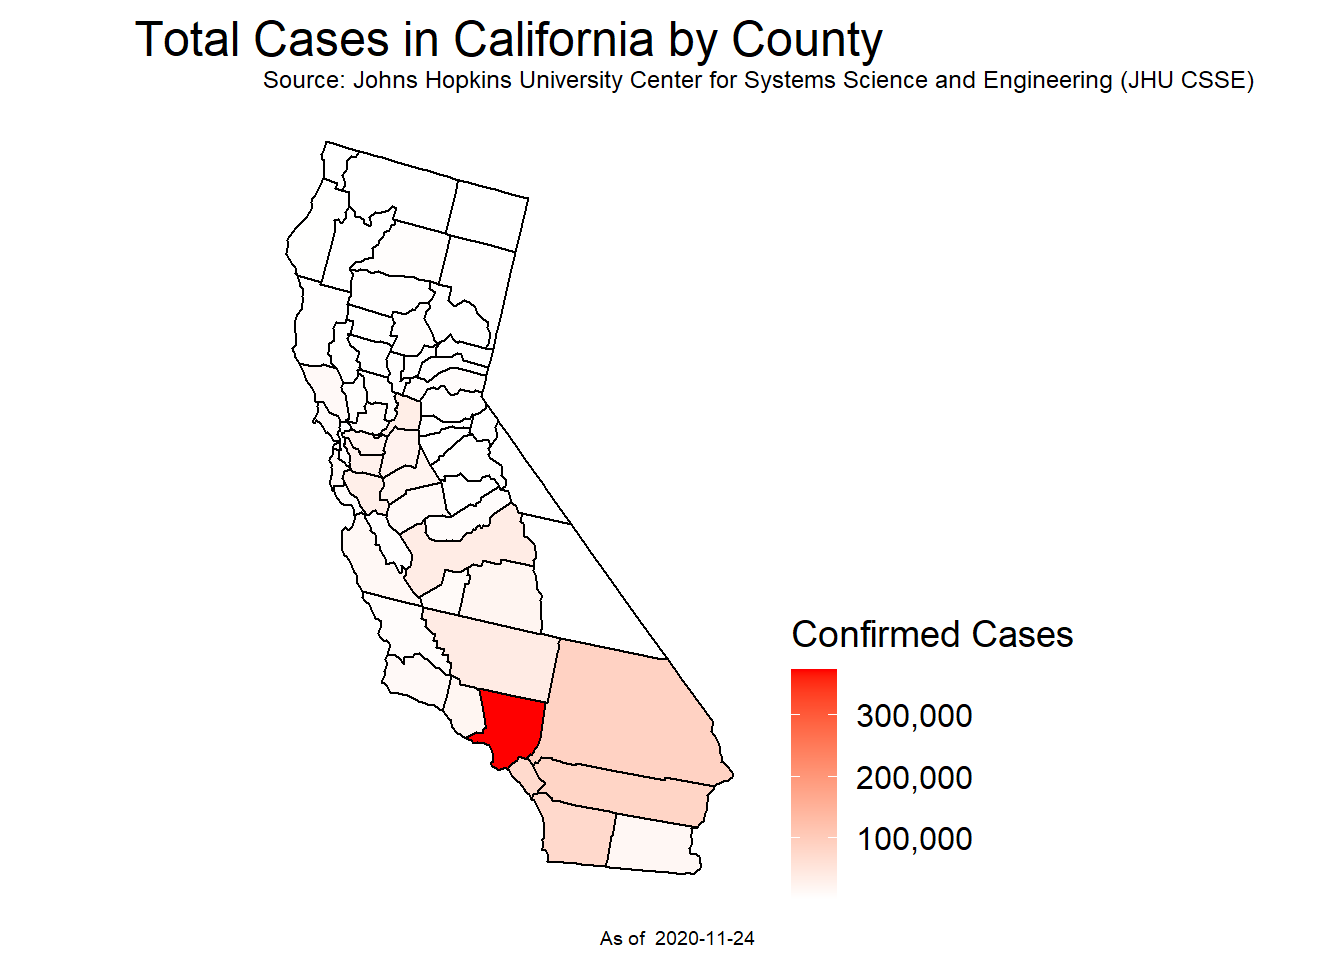
\includegraphics{FinalReport_files/figure-latex/unnamed-chunk-5-1.pdf}

As we see in \emph{Figure 4} Los Angeles county is by far the greatest
in size with over 10 million residents, along with Orange, San Diego,
San Bernadino, and Riverside counties as being the most dense for
population. Referencing my website will give interactive displays of
each county and the actual 2019 population estimates within. Population
can be a potential confounding variable for the relationship of air
quality on the number of covid cases. The more dense the county is in
population would call for more traffic and vechile smog pollution and
mamy vecotrs of spread ammongst people.

\hypertarget{enviornmental-protection-agency-epa-air-quality-index}{%
\subsection{Enviornmental Protection Agency (EPA) Air Quality
Index}\label{enviornmental-protection-agency-epa-air-quality-index}}

Preparing our Air Quality dataset to be merged with the US Census and
daily covid cases I wrangled and cleaned the data matching the Date
format. From the raw dataset I noticed that some counties have more
daily recorded measures of AQI and PM 2.5 than others. Some counties may
have had fewer daily recordings this year due to the virus leaving the
sites unmanned or even by the fires that heavily affected some of the
counties to have drastic AQI of over 500. In \emph{Figure 5} we see the
distribution of AQI for each county and can see the counties that have
extraneous outliers. Counties such as Mariposa with the Creek Fire and
Mono county with the Mountain View Fire. To account for the differences
I averaged the daily AQI and PM2.5 measures by day for some counties are
much larger than other and require more recording sites. Then I averaged
the AQI and PM2.5 measures again from all the single daily averages to
account for the size differences in counties.

\textbf{Figure 5: Air Quality Within California}
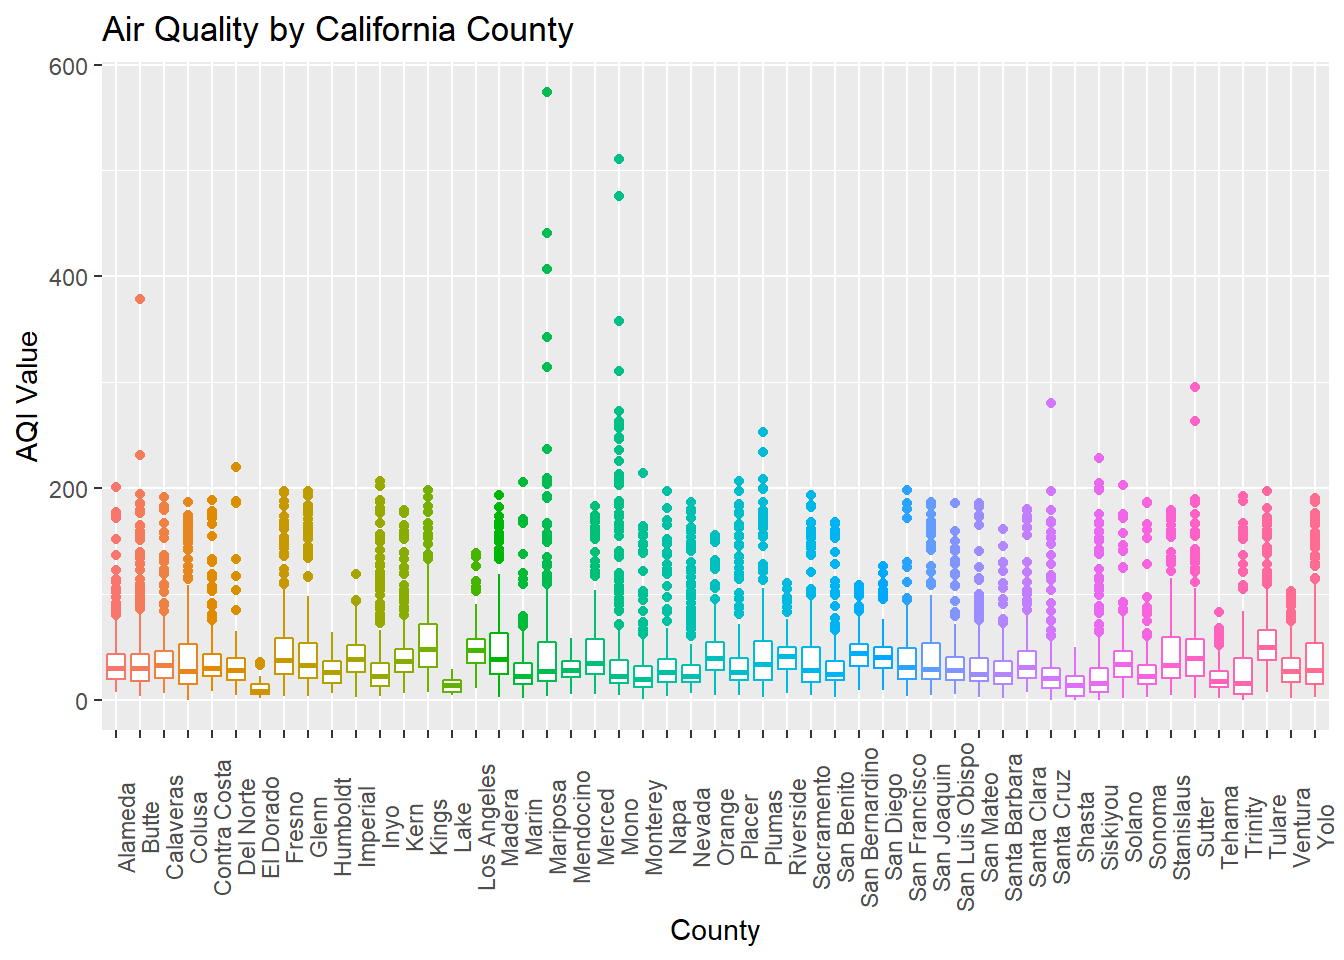
\includegraphics{FinalReport_files/figure-latex/AQI Visual-1.pdf}

\textbf{Figure 6: Combined Visuals}
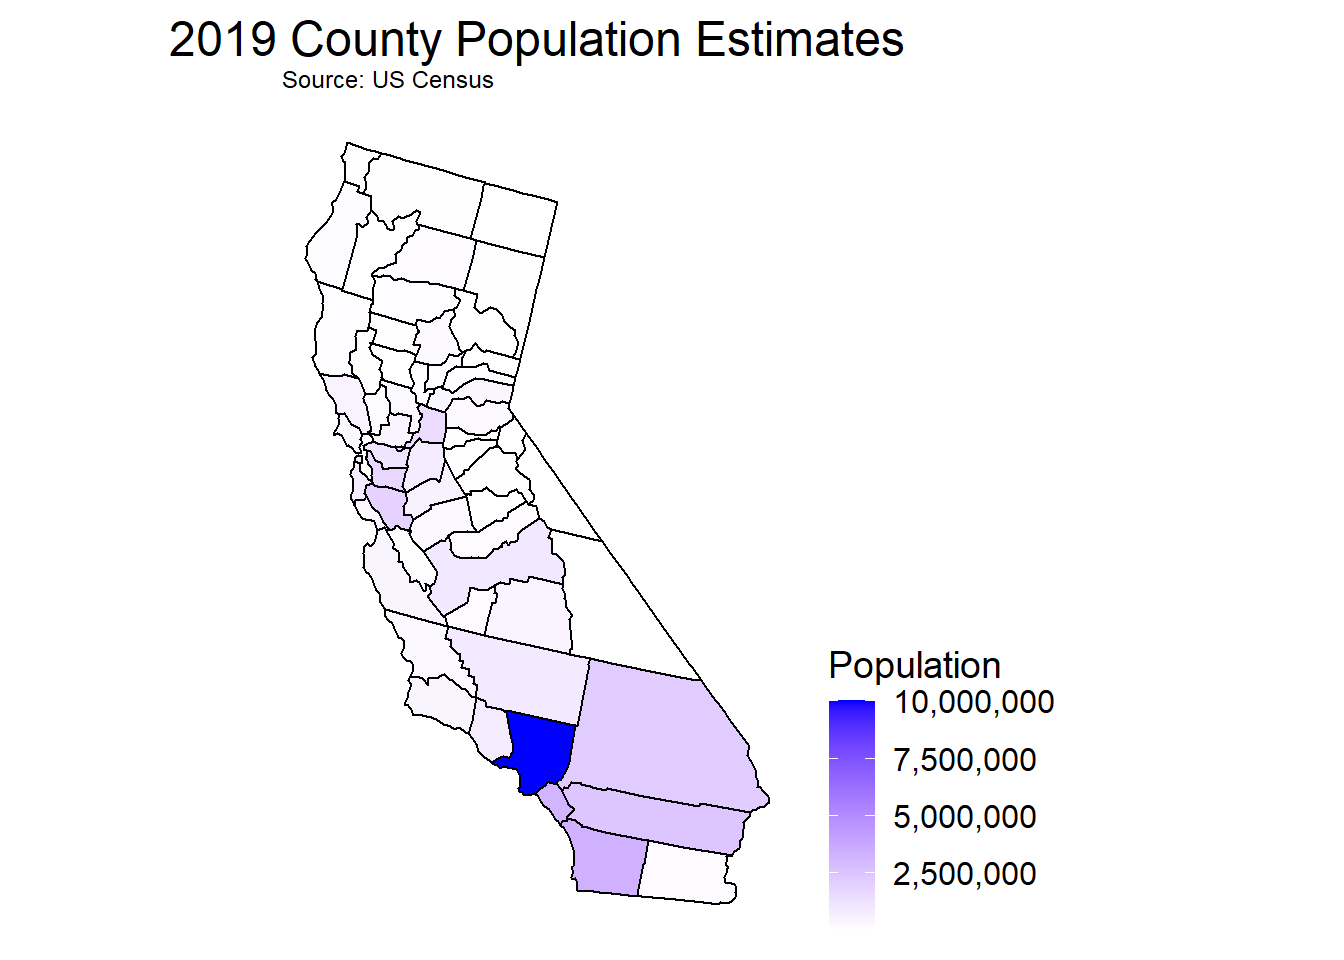
\includegraphics{FinalReport_files/figure-latex/unnamed-chunk-7-1.pdf}

In comparing the two datasets of Air Quality and Daily covid cases in
\emph{Figure 6} aligning the two graphs to give an overlay starting at
the beginning of the year with AQI and the start of the pandemic we see
interesting trends of a spike happening in both datasets during the
early days in the month of July most likely after the big holiday Fourth
of July. This also shows the affect of air pollution on the number of
covid cases as there were many fireworks shot in th sky contributing to
more PM 2.5 pollutants there was also an increase in cases. In my
website my interactive visual will give the actual number of AQI, covid
cases, and the date this all occured in Los Angeles county.

\textbf{Figure 7: Attack Rate of Covid Cases}
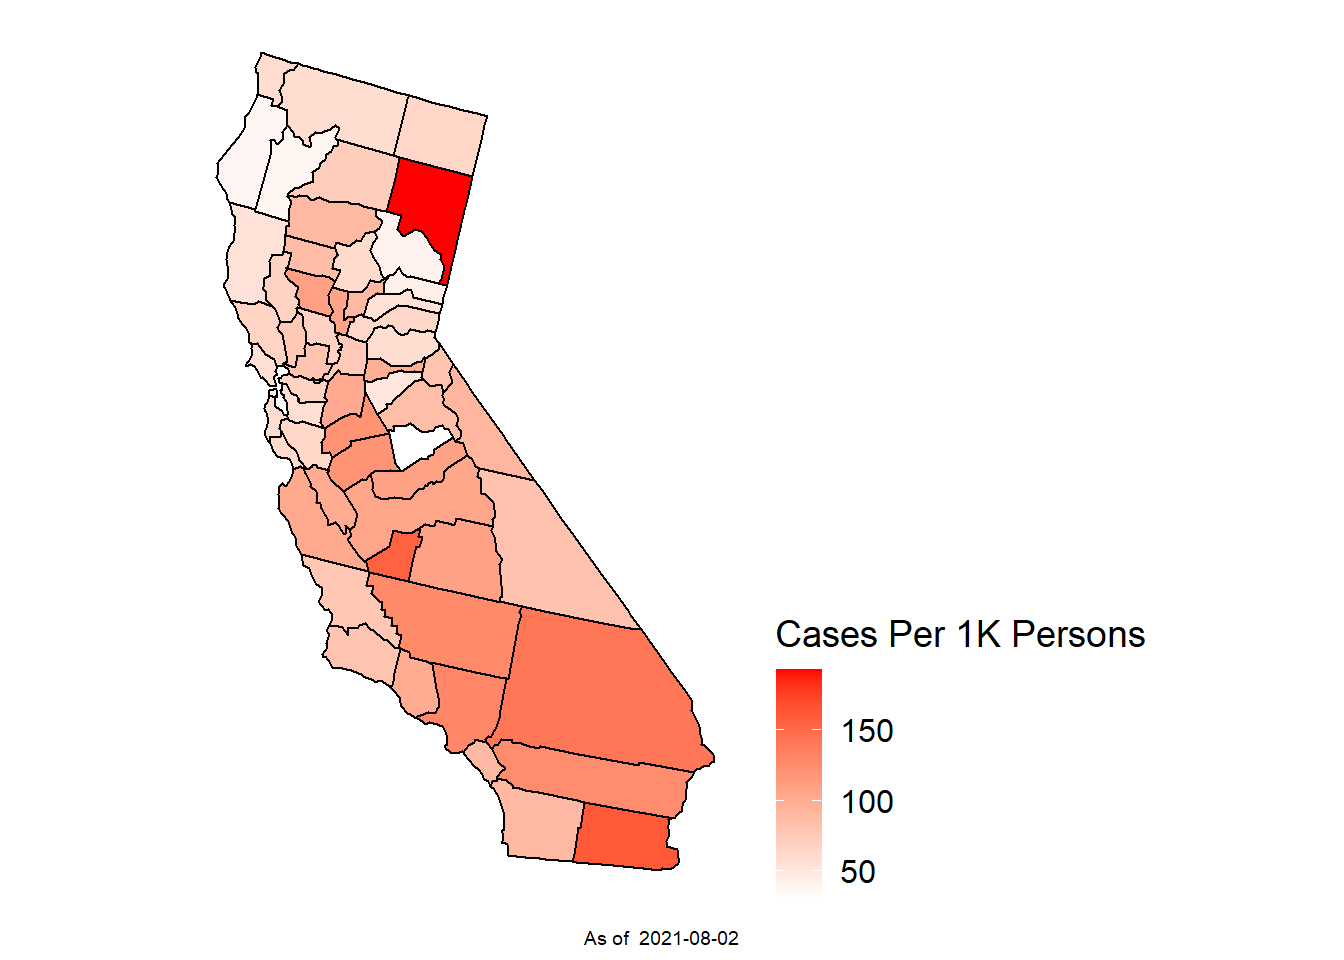
\includegraphics{FinalReport_files/figure-latex/unnamed-chunk-9-1.pdf}

One figure to draw attention to is \emph{Figure 7} I combined the two
datasets of the US Census data to get the \texttt{TOT\_POP} of each
county and daily covid cases to get the total number of prevalence cases
\texttt{Confirmed}. I normalized the attack rate of number of people
contracting covid by the population of the county,
\(\frac{\text{Confirmed}}{\text{TOT_POP}} \times 10000\) =
\texttt{rateper1k}. Creating a spatial density map of California by
county of the attack rate per 1,000 persons we can see how each county
is compared to each other when accounting for their population size. We
see that Imperial county has the highest attack rate of 85.9 per 1,000
persons and has a total population of 181,215, meaning that there would
be approximately 86 people out of 1,000 within Imperial county would
contract the corona virus. Also Kings county with an attack rate of 67
per 1,000 persons and has a total population of 152,940.

\textbf{Table 1: AQI County Categories}

\begin{longtable}[]{@{}lrrl@{}}
\toprule
County & Mean\_AQI & Mean\_PM2.5 & Category\tabularnewline
\midrule
\endhead
Alameda & 37.18892 & 10.889011 & Good\tabularnewline
Butte & 42.06522 & 14.658618 & Good\tabularnewline
Calaveras & 40.75768 & 12.478157 & Good\tabularnewline
Colusa & 40.78526 & 13.437233 & Good\tabularnewline
Contra Costa & 38.84119 & 11.257862 & Good\tabularnewline
Del Norte & 33.96471 & 10.150000 & Good\tabularnewline
El Dorado & 12.07500 & 2.862500 & Good\tabularnewline
Fresno & 47.22630 & 15.237381 & Good\tabularnewline
Glenn & 46.46885 & 15.869180 & Good\tabularnewline
Humboldt & 27.94366 & 6.743662 & Good\tabularnewline
Imperial & 39.92153 & 10.354000 & Good\tabularnewline
Inyo & 35.71946 & 12.180047 & Good\tabularnewline
Kern & 44.05202 & 13.409081 & Good\tabularnewline
Kings & 56.62305 & 17.882970 & Moderate\tabularnewline
Lake & 14.13333 & 3.366667 & Good\tabularnewline
Los Angeles & 48.33325 & 13.438065 & Good\tabularnewline
Madera & 49.52025 & 15.810436 & Good\tabularnewline
Marin & 30.48742 & 8.688050 & Good\tabularnewline
Mariposa & 48.19355 & 20.426935 & Good\tabularnewline
Mendocino & 29.25824 & 7.152747 & Good\tabularnewline
Merced & 47.01429 & 14.500476 & Good\tabularnewline
Mono & 50.29063 & 25.836542 & Moderate\tabularnewline
Monterey & 27.50492 & 8.249094 & Good\tabularnewline
Napa & 34.40777 & 10.017152 & Good\tabularnewline
Nevada & 33.50415 & 10.272819 & Good\tabularnewline
Orange & 43.73240 & 11.821170 & Good\tabularnewline
Placer & 38.48873 & 12.427343 & Good\tabularnewline
Plumas & 47.60139 & 17.828562 & Good\tabularnewline
Riverside & 40.65813 & 10.809516 & Good\tabularnewline
Sacramento & 40.49550 & 12.668012 & Good\tabularnewline
San Benito & 33.17619 & 9.332381 & Good\tabularnewline
San Bernardino & 44.25559 & 11.949591 & Good\tabularnewline
San Diego & 41.14893 & 10.830919 & Good\tabularnewline
San Francisco & 37.11250 & 10.660312 & Good\tabularnewline
San Joaquin & 42.22723 & 13.200285 & Good\tabularnewline
San Luis Obispo & 33.17909 & 9.243970 & Good\tabularnewline
San Mateo & 34.12893 & 9.866667 & Good\tabularnewline
Santa Barbara & 29.43758 & 7.745347 & Good\tabularnewline
Santa Clara & 38.33954 & 11.049689 & Good\tabularnewline
Santa Cruz & 28.55901 & 9.272516 & Good\tabularnewline
Shasta & 15.78571 & 3.897143 & Good\tabularnewline
Siskiyou & 28.66978 & 9.896262 & Good\tabularnewline
Solano & 39.96406 & 11.585313 & Good\tabularnewline
Sonoma & 28.98413 & 8.175238 & Good\tabularnewline
Stanislaus & 44.64271 & 13.793594 & Good\tabularnewline
Sutter & 48.65823 & 16.009019 & Good\tabularnewline
Tehama & 22.52941 & 5.578235 & Good\tabularnewline
Trinity & 31.33333 & 10.232292 & Good\tabularnewline
Tulare & 58.32914 & 18.357986 & Moderate\tabularnewline
Ventura & 30.46444 & 7.826894 & Good\tabularnewline
Yolo & 41.51398 & 13.209627 & Good\tabularnewline
\bottomrule
\end{longtable}

\hypertarget{results}{%
\section{Results}\label{results}}

\textbf{Table 2: Preliminary Poisson Model}

\begin{longtable}[]{@{}lrrrr@{}}
\toprule
parameter & rr & 2.5 \% & 97.5 \% & pvalue\tabularnewline
\midrule
\endhead
(Intercept) & 0.0003167 & 0.0002753 & 0.0003642 & 0\tabularnewline
TOT\_MALE & 0.9999884 & 0.9999875 & 0.9999893 & 0\tabularnewline
TOT\_FEMALE & 0.9999884 & 0.9999876 & 0.9999893 & 0\tabularnewline
White & 1.0000124 & 1.0000114 & 1.0000133 & 0\tabularnewline
Black & 1.0000141 & 1.0000131 & 1.0000151 & 0\tabularnewline
Hispanic & 0.9999993 & 0.9999992 & 0.9999994 & 0\tabularnewline
Asian & 1.0000115 & 1.0000106 & 1.0000124 & 0\tabularnewline
Other & 1.0000099 & 1.0000083 & 1.0000115 & 0\tabularnewline
pct\_19 & 4900.2000395 & 4113.1311092 & 5837.8786841 & 0\tabularnewline
pct\_2064 & 24.0052745 & 19.5794783 & 29.4314892 & 0\tabularnewline
avgAQI & 1.0372287 & 1.0355150 & 1.0389452 & 0\tabularnewline
avgPM2.5 & 0.9174265 & 0.9134849 & 0.9213851 & 0\tabularnewline
\bottomrule
\end{longtable}

\textbf{Table 3: Final Negative Binomial Model}

\begin{longtable}[]{@{}lrrrr@{}}
\toprule
parameter & rr & 2.5 \% & 97.5 \% & pvalue\tabularnewline
\midrule
\endhead
(Intercept) & 6.920000e-05 & 0.0000108 & 4.438000e-04 &
0.0000000\tabularnewline
TOT\_MALE & 9.999886e-01 & 0.9999608 & 1.000016e+00 &
0.4221403\tabularnewline
TOT\_FEMALE & 9.999833e-01 & 0.9999528 & 1.000014e+00 &
0.2846207\tabularnewline
White & 1.000015e+00 & 0.9999850 & 1.000046e+00 &
0.3203241\tabularnewline
Black & 1.000018e+00 & 0.9999845 & 1.000051e+00 &
0.2957155\tabularnewline
Hispanic & 9.999988e-01 & 0.9999955 & 1.000002e+00 &
0.4832566\tabularnewline
Asian & 1.000014e+00 & 0.9999846 & 1.000043e+00 &
0.3524272\tabularnewline
Other & 1.000003e+00 & 0.9999483 & 1.000058e+00 &
0.9096048\tabularnewline
pct\_19 & 5.365662e+04 & 2628.9814689 & 1.095113e+06 &
0.0000000\tabularnewline
pct\_2064 & 1.866367e+02 & 7.8520901 & 4.436174e+03 &
0.0012174\tabularnewline
avgAQI & 9.995592e-01 & 0.9738794 & 1.025916e+00 &
0.9735132\tabularnewline
avgPM2.5 & 1.013048e+00 & 0.9576485 & 1.071651e+00 &
0.6514247\tabularnewline
\bottomrule
\end{longtable}

In combing all three datasets of daily covid cases, EPA daily air
quality data, and the US Census of demogrpahic populations I decided to
run a poisson model running a full model with all my variables included
as \texttt{Confirmed} cases as my predicted y variable \(\hat{y}\). A
Poisson model would be most appropriate because the count data of
confirmed cases is strictly {[}0, \(\infty\)) as our other variables as
well, with the Poisson model I can also include an offset variable of
\texttt{TOT\_POP} to normalize every county in California to obtain the
attack rate. The first Poisson model ran with all variables being
statistically significant with a p-value less than our significance
level of 0.05. However, \texttt{pct\_65over} was not statistically
significant and I continued the next model exluding this variable. We
find in \emph{Table 2} the relative ratios for all the variables except
for \texttt{pct\_19} and \texttt{pct\_2064} are relatively null. Meaning
that the percentage of age groups 19 and younger, and 20 to 64 are at a
much higher risk of contracting covid. The AIC for the Poisson model is
19757 which is extremly high and does not compare well with other models
if they were to have a lower AIC, as a lower value would indicate a
better fit. Another measure of checking our model's fit is the
dispersion test \(H_0: \tau = 0\) and \(H_a: \tau \ne 0\), our model has
a dispersion of 408.63 and a p-value of 0.0013 which rejects the null
hypothesis and we can conclude that there is overdispersion.

Oversidpersion would cause our model to have smaller significance in our
paramters as our p-value would be smaller and cause our estimated
standard errors to be smaller than what is true. A Negative Binomial
model would account for such an overdispersion and we see an improvement
in our full model excluding \texttt{pct\_65over} with the offset of
\texttt{TOT\_POP} as our AIC value is much lower at 917.30 with our
\(\theta = 12.63\). In testing our model's goodness of fit, the deviance
GOF test does not show any departure from good fit as our p-value is not
significant with a value of 0.0856.

\hypertarget{discussion}{%
\section{Discussion}\label{discussion}}

The year 2020 will forever be memorable with all the more peculiar as
the US Census was administered and I believe we will have better
accounts of the true population in 2020 compared to the algorithm
generated 2019 population estimate and even more hidden trends
discovered. For future notes on running this model with the 2020 US
Census day would be to administer interaction effects for the age groups
and race to see if its significant in its relation with attack ratio of
corona virus. I would include other variables such as population density
per square mile to get the idea of how crowded or spacious other
counties are with their populations and with the closer proximity of
people how that effects the attack ratio of contracting covid. Also to
get a better understanding of how air pollution directly relates to the
contracting of the virus to include a lag time of 14 days when a patient
was diagnosed with the virus and comparing the air quality 14 days prior
of their diagnostic screening.

\end{document}
